\documentclass[11pt]{article}

\usepackage{tikz}
\usepackage{environ}

\usetikzlibrary{
    datavisualization.formats.functions,
    decorations,
    positioning,
    fit,
    shapes.geometric, % To use regular polygons as shapes
    calc
}

\tikzset{
    hexagon/.style = {
        regular polygon,
        regular polygon sides = 6,
        draw,
        minimum size = #1
    }
}

\begin{document}

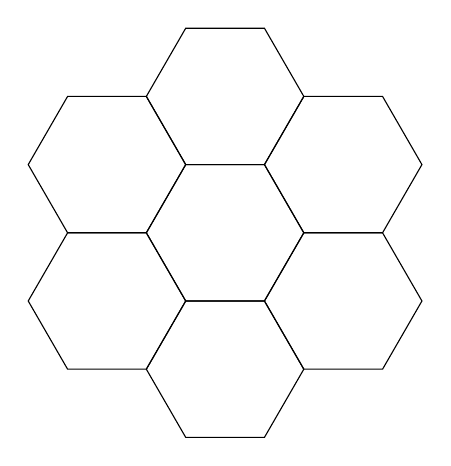
\begin{tikzpicture}
    \def\hdiam{2}
    \node[hexagon = \hdiam cm] at (0, 0) {};
    \pgfmathparse{\hdiam * cos(30)}
    \foreach \ang in {30, 90, ..., 330} {
        \node[hexagon = \hdiam cm] at (\ang:\pgfmathresult cm) {};
    }

\end{tikzpicture}

\end{document}
